\subsection{Анализ цепи во временной области}\label{sec:analysis}

Исходная цепь представлена на рис. \ref{fig:circ_source}

\begin{figure}[H]
    \centering
    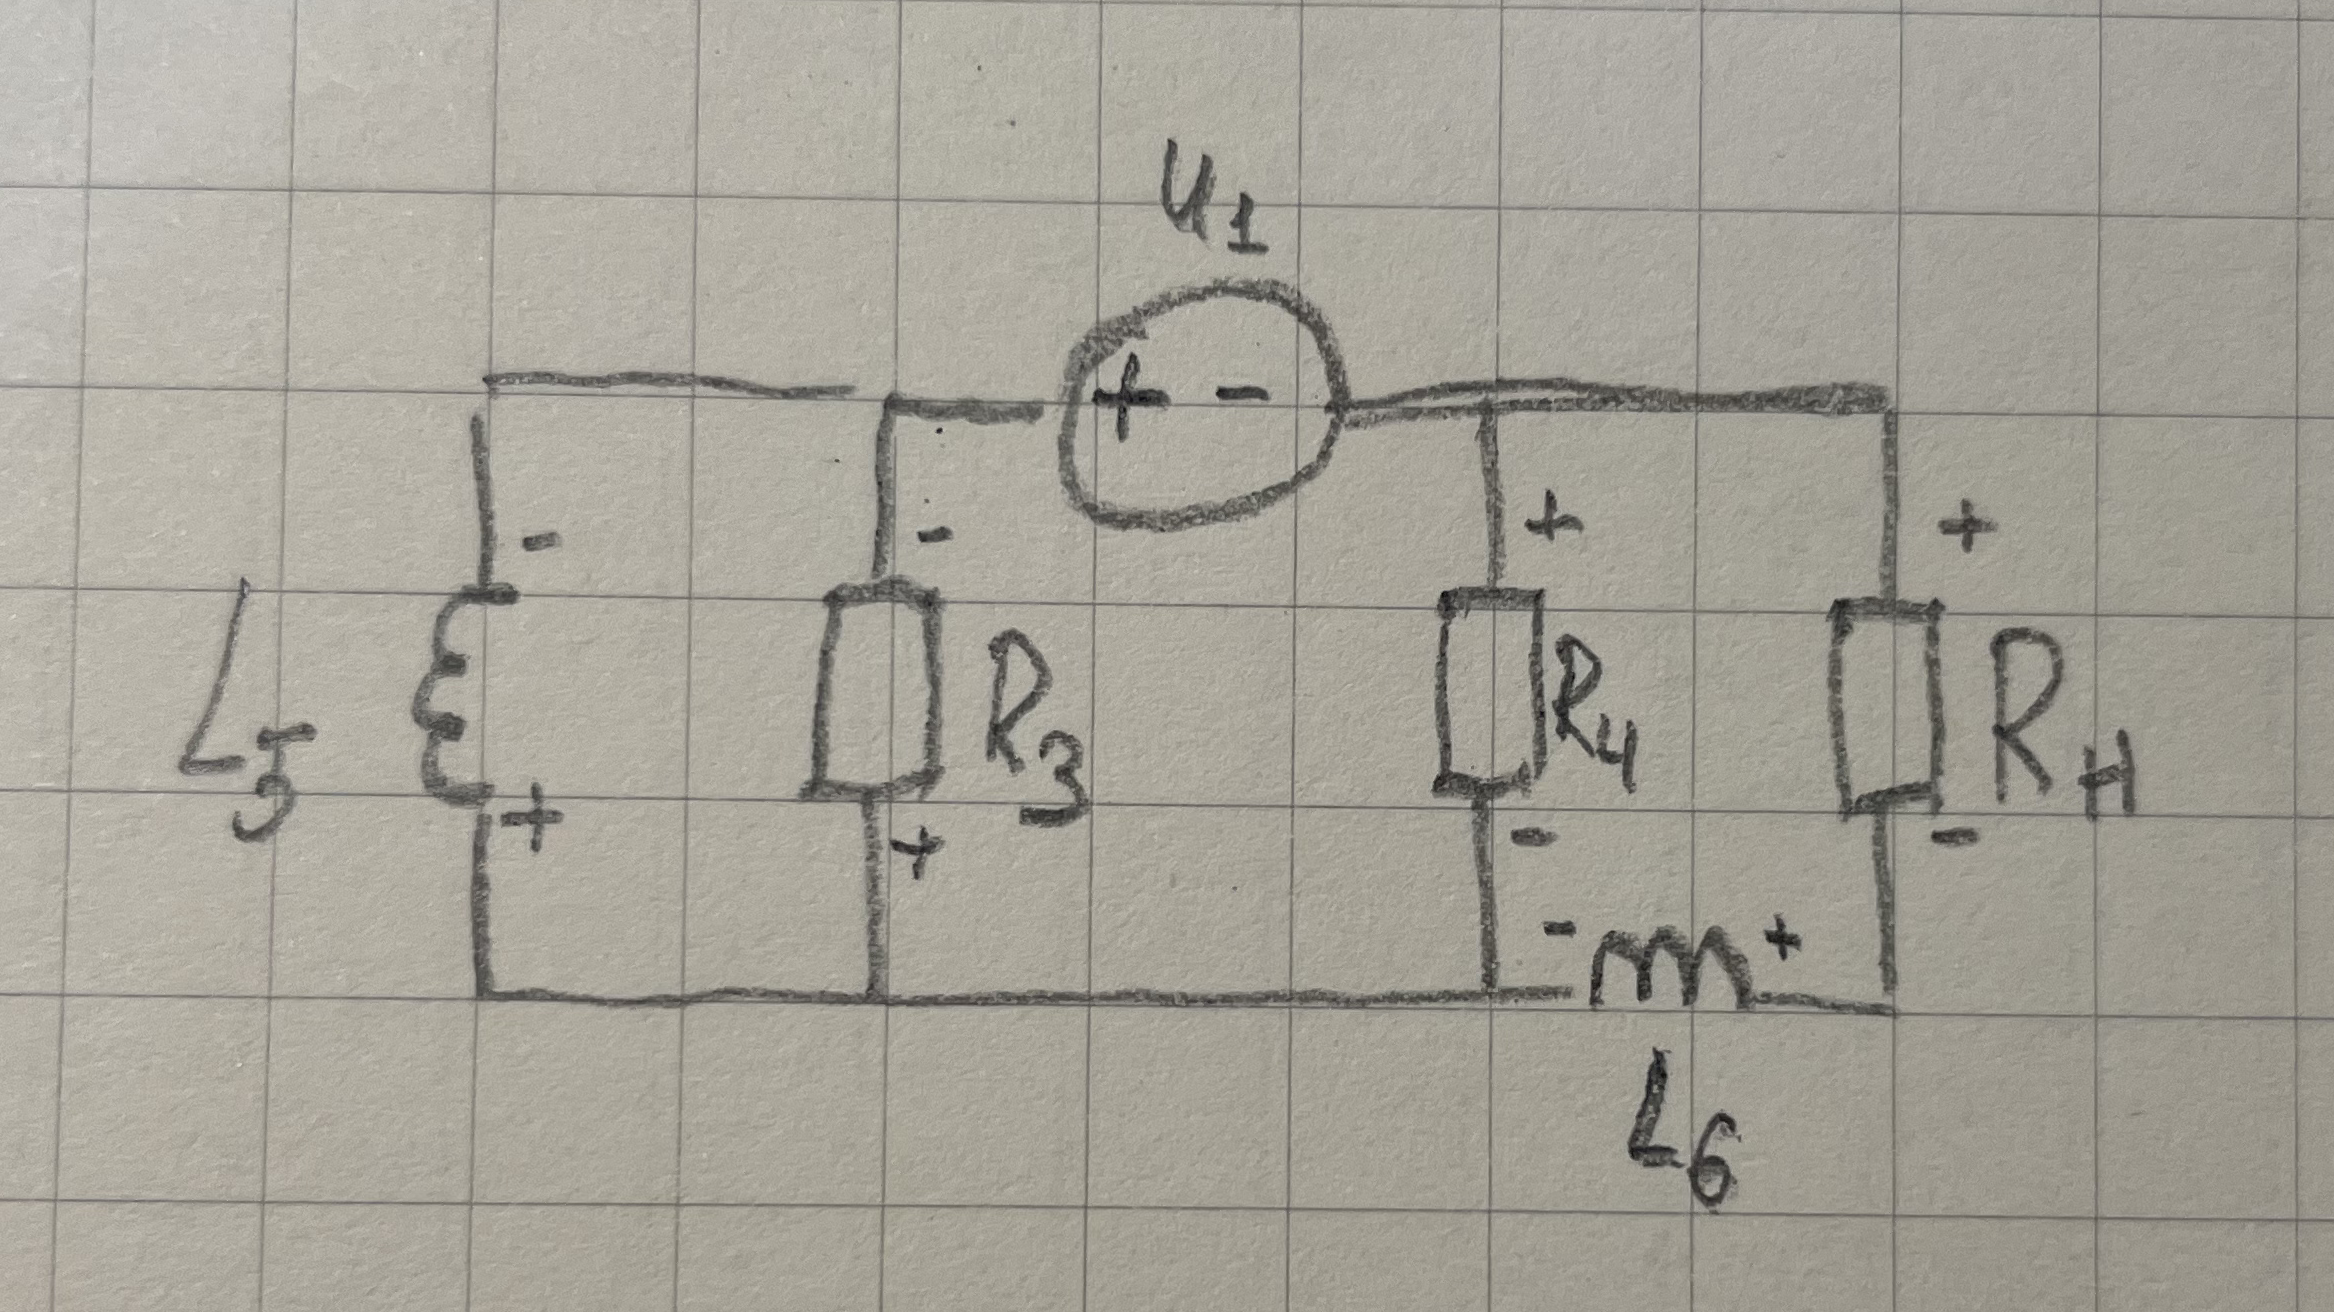
\includegraphics[width=0.7\linewidth]{photo/circ_source}
    \caption{Исходная цепь}
    \label{fig:circ_source}
\end{figure}

По условию:

$ u_1 = 1 $

$ R_н = 1  $

$ R_3 = 2 $

$ R_4 = 2 $

$ L_5 = 0.5 $

$ L_6 = 1 $

Запишем систему уравнений состояния цепи:

\begin{equation}\label{eq:state}
    \begin{cases}
        \dfrac{di_{L_5}}{dt} = \dfrac{1}{L_5} u_{L_5}\\\\
        \dfrac{di_{L_6}}{dt} = \dfrac{1}{L_6} u_{L_6}\\
    \end{cases}
\end{equation}

Построим схему замещения цепи 
($ t > 0, L = ИТ $) 
(рис. \ref{fig:circ_replaced_1})

\begin{figure}[H]
    \centering
    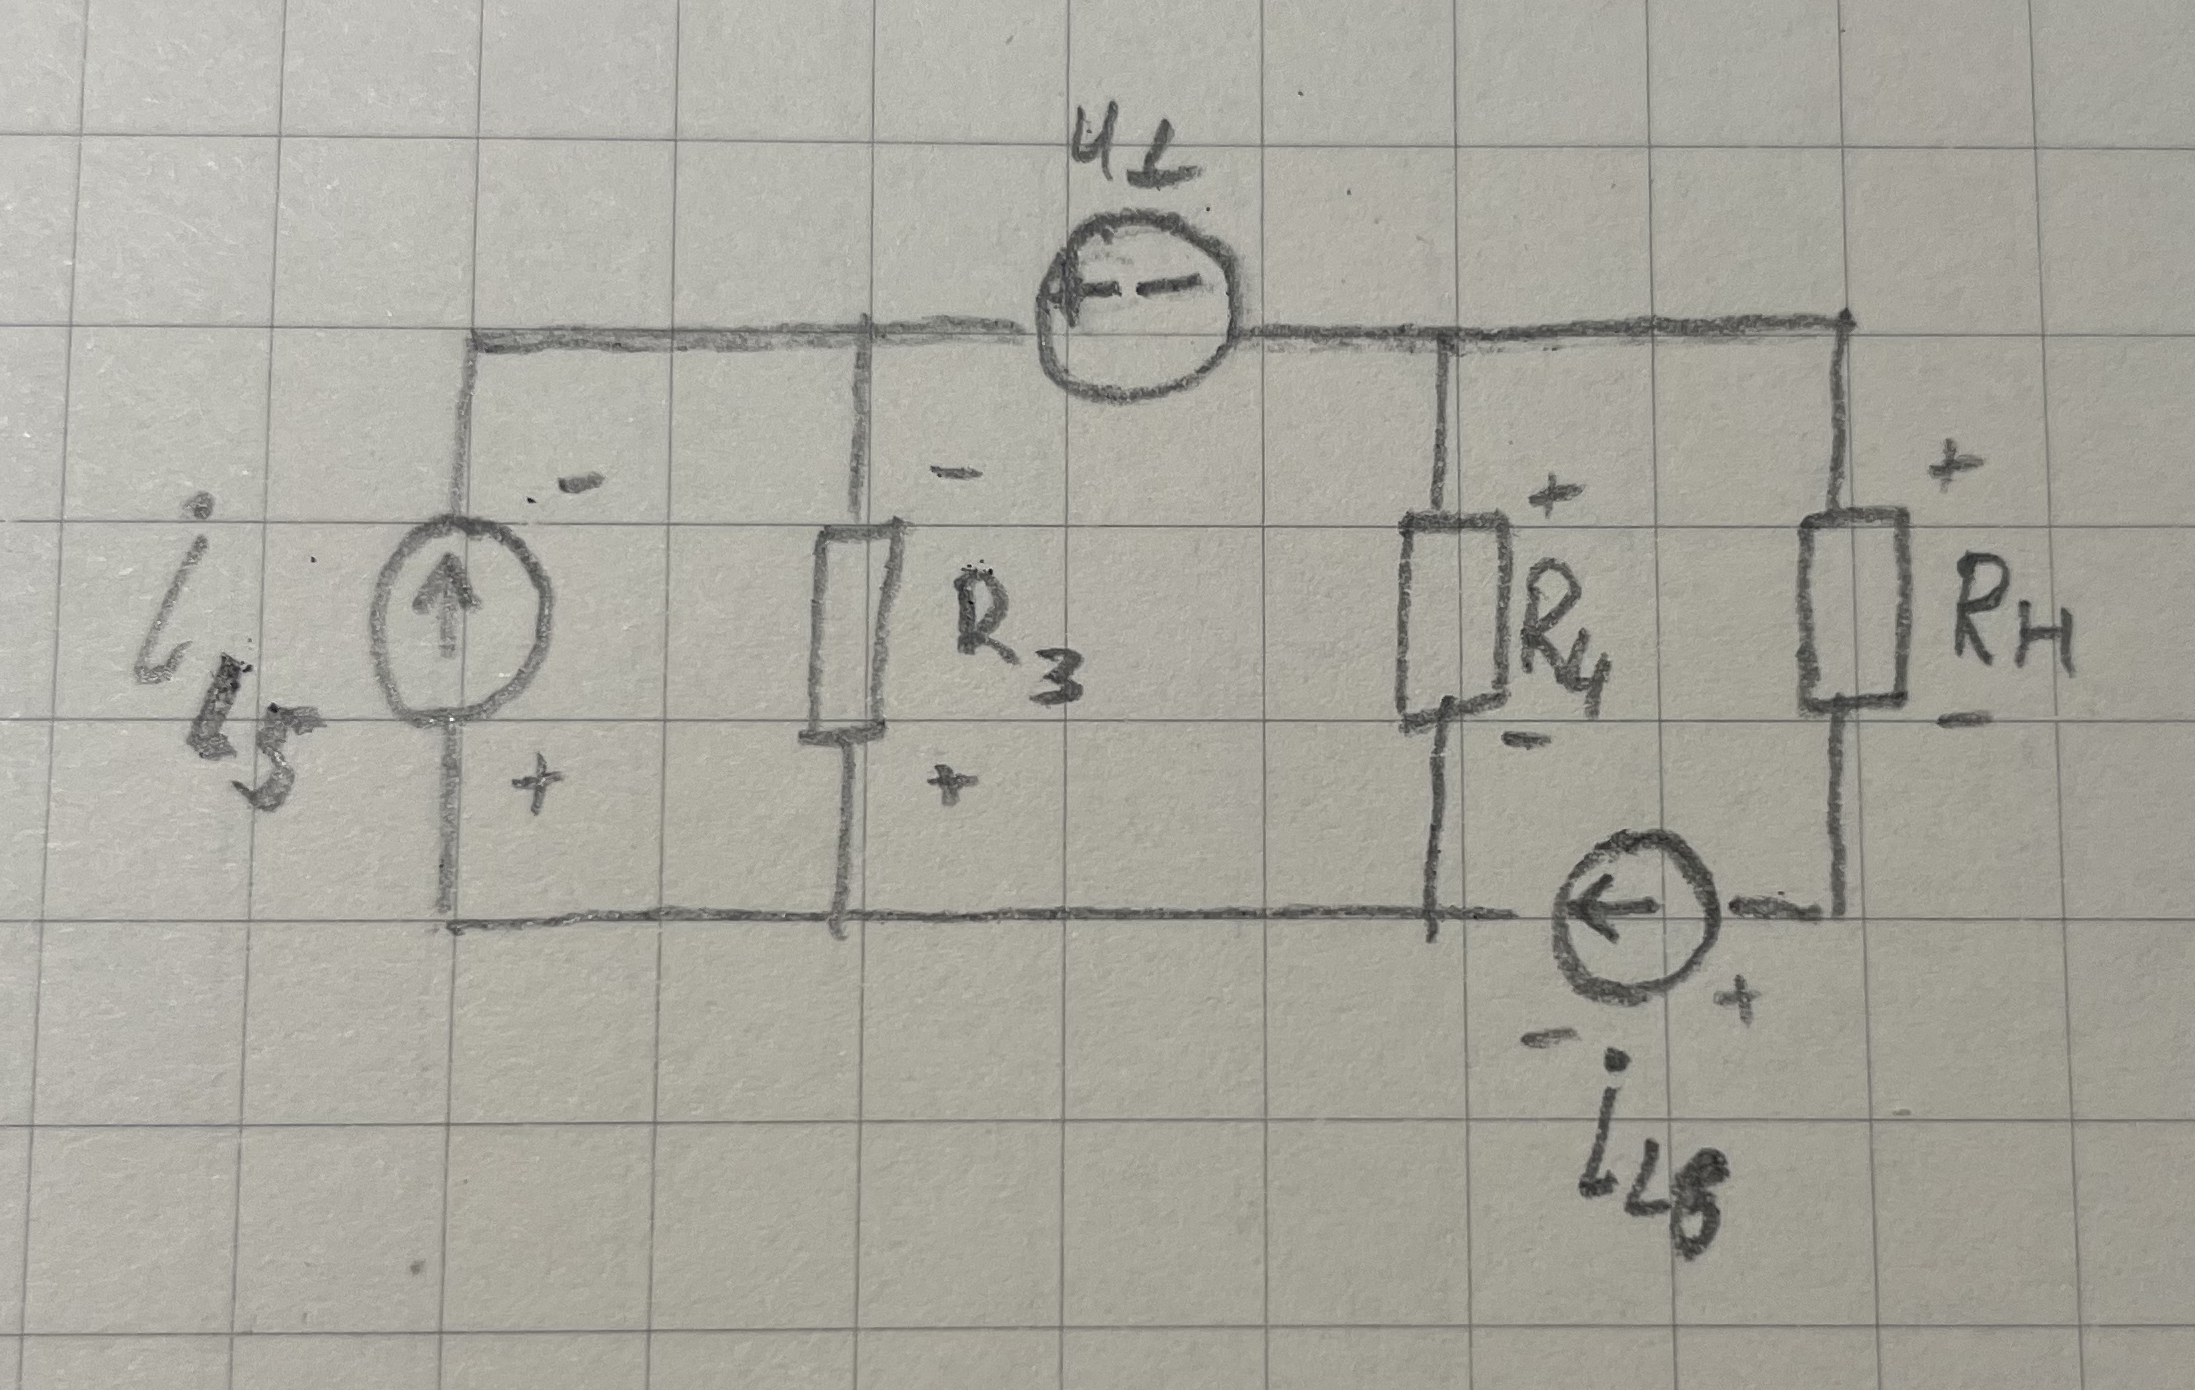
\includegraphics[width=0.7\linewidth]{photo/circ_replaced_1}
    \caption{Схема замещения. $ t > 0 $}
    \label{fig:circ_replaced_1}
\end{figure}

С помощью метода наложения выразим 
$ u_{L_5}, u_{L_6} $ из (\ref{eq:state})
через источники.

\begin{enumerate}
    \item Из схемы замещения на рис. \ref{fig:circ_overlay_1}:
    
    \begin{figure}[H]
        \centering
        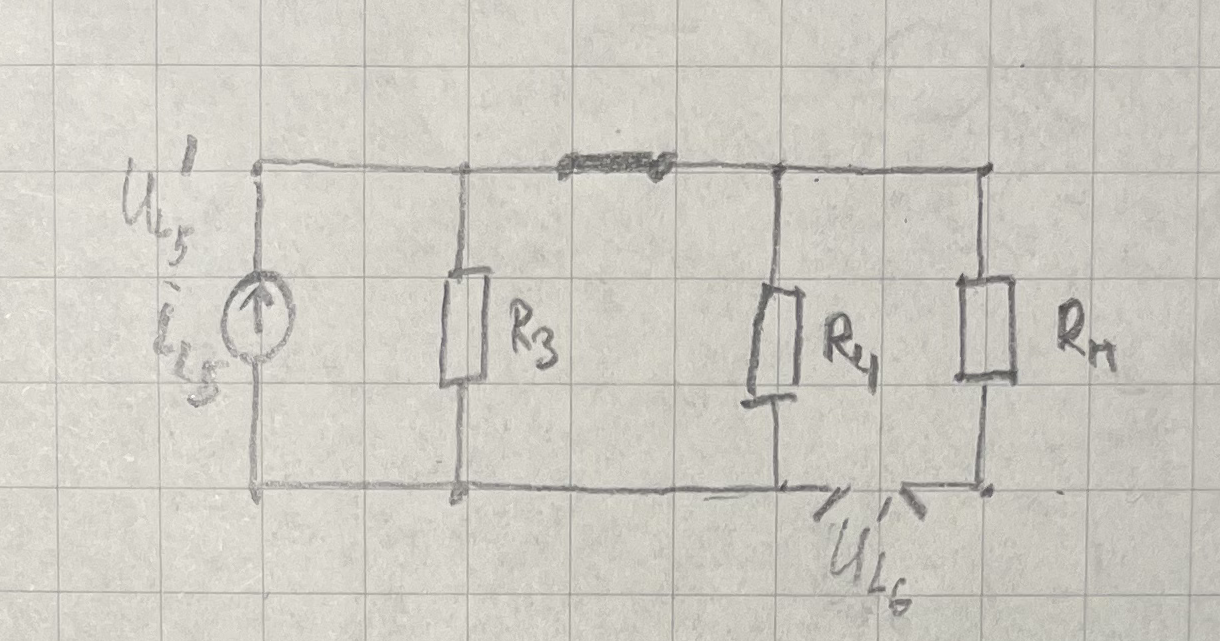
\includegraphics[width=0.7\linewidth]{photo/circ_overlay_1}
        \caption{Метод наложения - 1}
        \label{fig:circ_overlay_1}
    \end{figure}
    
    $ u'_{L_5} = 
    \dfrac{R_3 + R_4}{R_3 R_4} i_{L_5} = 
    \dfrac{2 + 2}{2 \times 2} i_{L_5} =
    i_{L_5}
    $
    
    $ u'_{L_6} = - u_{R_4} = - u_{R_3} = - i_{L_5} $
    
    \item Из схемы замещения на рис. \ref{fig:circ_overlay_2}:
    
    \begin{figure}[H]
        \centering
        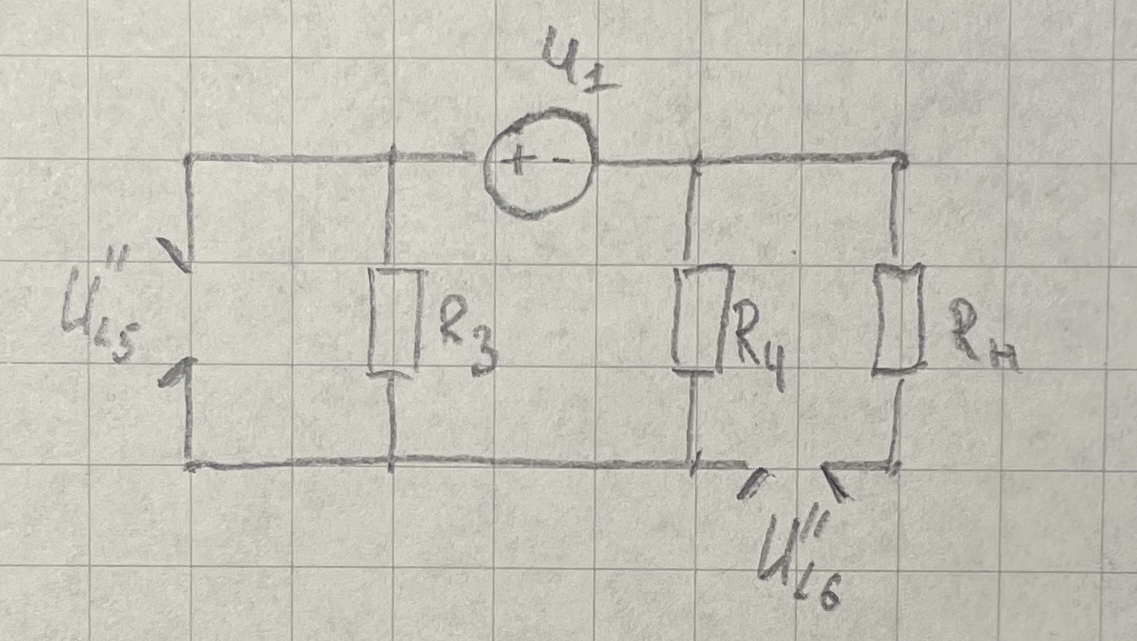
\includegraphics[width=0.7\linewidth]{photo/circ_overlay_2}
        \caption{Метод наложения - 2}
        \label{fig:circ_overlay_2}
    \end{figure}
    
    $ u''_{L_5} = 
    u_{R_3} = 
    R_3 \times i_{R_3} = 
    R_3 \times \dfrac{u_1}{R_3 + R_4} = 
    2 \times \dfrac{1}{2 + 2} = 
    0.5
    $
    
    $ u''_{L_6} = 
    - u_{R_4} =  
    - R_4 \times i_{R_4} = 
    - R_4 \times \dfrac{u_1}{R_3 + R_4} = 
    - 2 \times \dfrac{1}{2 + 2} = 
    - 0.5
    $
    
    \item Из схемы замещения на рис. \ref{fig:circ_overlay_3}:
    
    \begin{figure}[H]
        \centering
        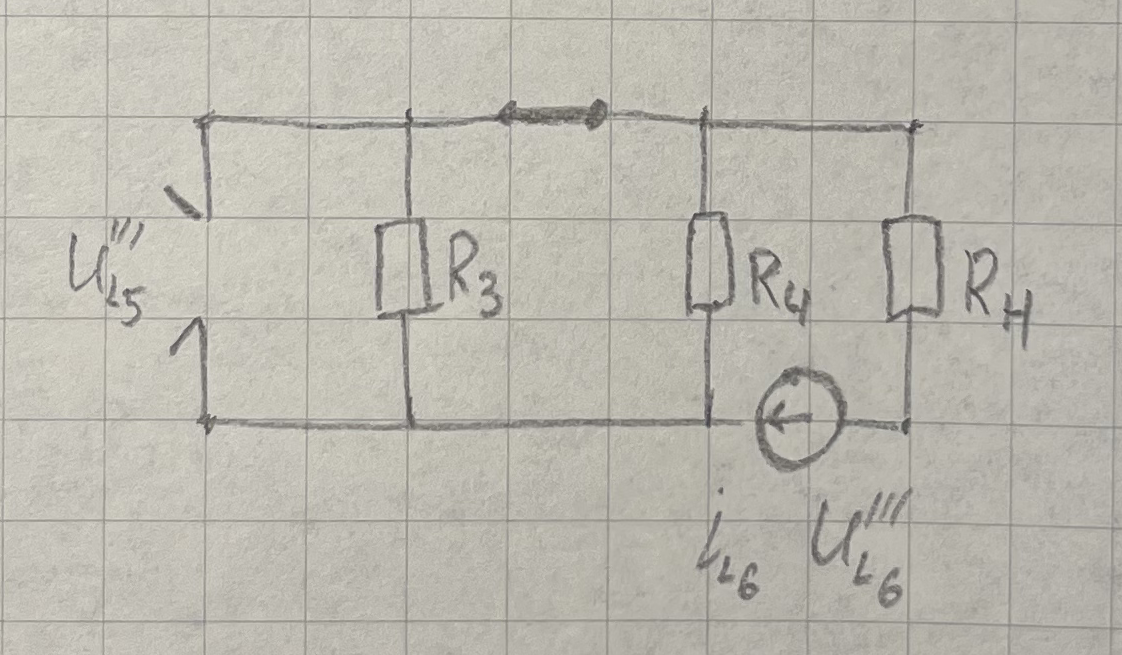
\includegraphics[width=0.7\linewidth]{photo/circ_overlay_3}
        \caption{Метод наложения - 3}
        \label{fig:circ_overlay_3}
    \end{figure}
    
    $ u'''_{L_5} = 
    u_{R_3} =
    R_3 \times i_{R_3} =
    R_3 \times \dfrac{1}{2} i_{L_6} =
    2 \times \dfrac{1}{2} i_{L_6} =
    i_{L_6}
    $
    
    $ u'''_{L_6} = 
    R_{вх} * i_{L_6} = 
    (\dfrac{R_3 + R_4}{R_3 \times R_4} + R_н) * i_{L_6} = 
    (\dfrac{2 + 2}{2 \times 2} + 1) * i_{L_6} = 
    2i_{L_6}
    $
\end{enumerate}

Итого:

$ u_{L_5} = 
u'_{L_5} + u''_{L_5} + u'''_{L_5} = 
i_{L_5} + 0.5 + i_{L_6} =
i_{L_5} + i_{L_6} + 0.5 $

$ u_{L_6} = 
u'_{L_6} + u''_{L_6} + u'''_{L_6} = 
- i_{L_5} - 0.5 + 2i_{L_6} =
- i_{L_5} + 2i_{L_6} - 0.5 $

\begin{equation}\label{eq:u_L_5}
u_{L_5} = 
i_{L_5} + i_{L_6} + 0.5
\end{equation}

\begin{equation}\label{eq:u_L_6}
u_{L_6} = 
- i_{L_5} + 2i_{L_6} - 0.5
\end{equation}

Подставим 
(\ref{eq:u_L_5}) и (\ref{eq:u_L_6}) в (\ref{eq:state}):

$$
\begin{cases}
    \dfrac{di_{L_5}}{dt} = \dfrac{1}{L_5} u_{L_5} =
    \dfrac{1}{0.5} (i_{L_5} + i_{L_6} + 0.5) =
    2i_{L_5} + 2i_{L_6} + 1
    \\\\
    \dfrac{di_{L_6}}{dt} = \dfrac{1}{L_6} u_{L_6} =
    \dfrac{1}{1} (- i_{L_5} + 2i_{L_6} - 0.5) =
    - i_{L_5} + 2i_{L_6} - 0.5
    \\
\end{cases}
$$

Найдём корни характеристического уравнения:\\

$ |A| - p|E| = 0 $
\\

$ 
\begin{vmatrix}
2 & 2\\
-1 & 2
\end{vmatrix}
-
\begin{vmatrix}
p & 0\\
0 & p
\end{vmatrix} =
\begin{vmatrix}
2 - p & 2\\
-1 & 2 - p
\end{vmatrix} = 
(2 - p)^2 - 2(-1) = 
p^2 - 4p + 4 + 2
$\\\\

$ p^2 - 4p + 6 = 0 $\\

$ p_{1,2} = 
\dfrac{4 \pm \sqrt{(-4)^2 - 4 \cdot 1 \cdot 6}}{2} = 
\dfrac{4 \pm \sqrt{8j^2}}{2} =
2 \pm \sqrt{2}j
$\\

Полученные корни:

\begin{equation}\label{eq:p_roots}
    p_{1,2} = 2 \pm \sqrt{2}j
\end{equation}

Корни комплексные.
Значит, свободные составляющие
будут такими:

$ i_{L_5 св.}(t) = 
A_1 e^{2t} \cos(t\sqrt{2}) + 
A_2 e^{2t} \sin(t\sqrt{2}) 
$

$ i_{L_6 св.}(t) = 
B_1 e^{2t} \cos(t\sqrt{2}) + 
B_2 e^{2t} \sin(t\sqrt{2}) 
$\\

Найдём установившиеся (вынужденные) составляющие
$ i_{L_5 уст.} $ и $ i_{L_6 уст.} $
($ t \rightarrow \infty, L = КЗ $)
(рис. \ref{fig:circ_replaced_2})

\begin{figure}[H]
    \centering
    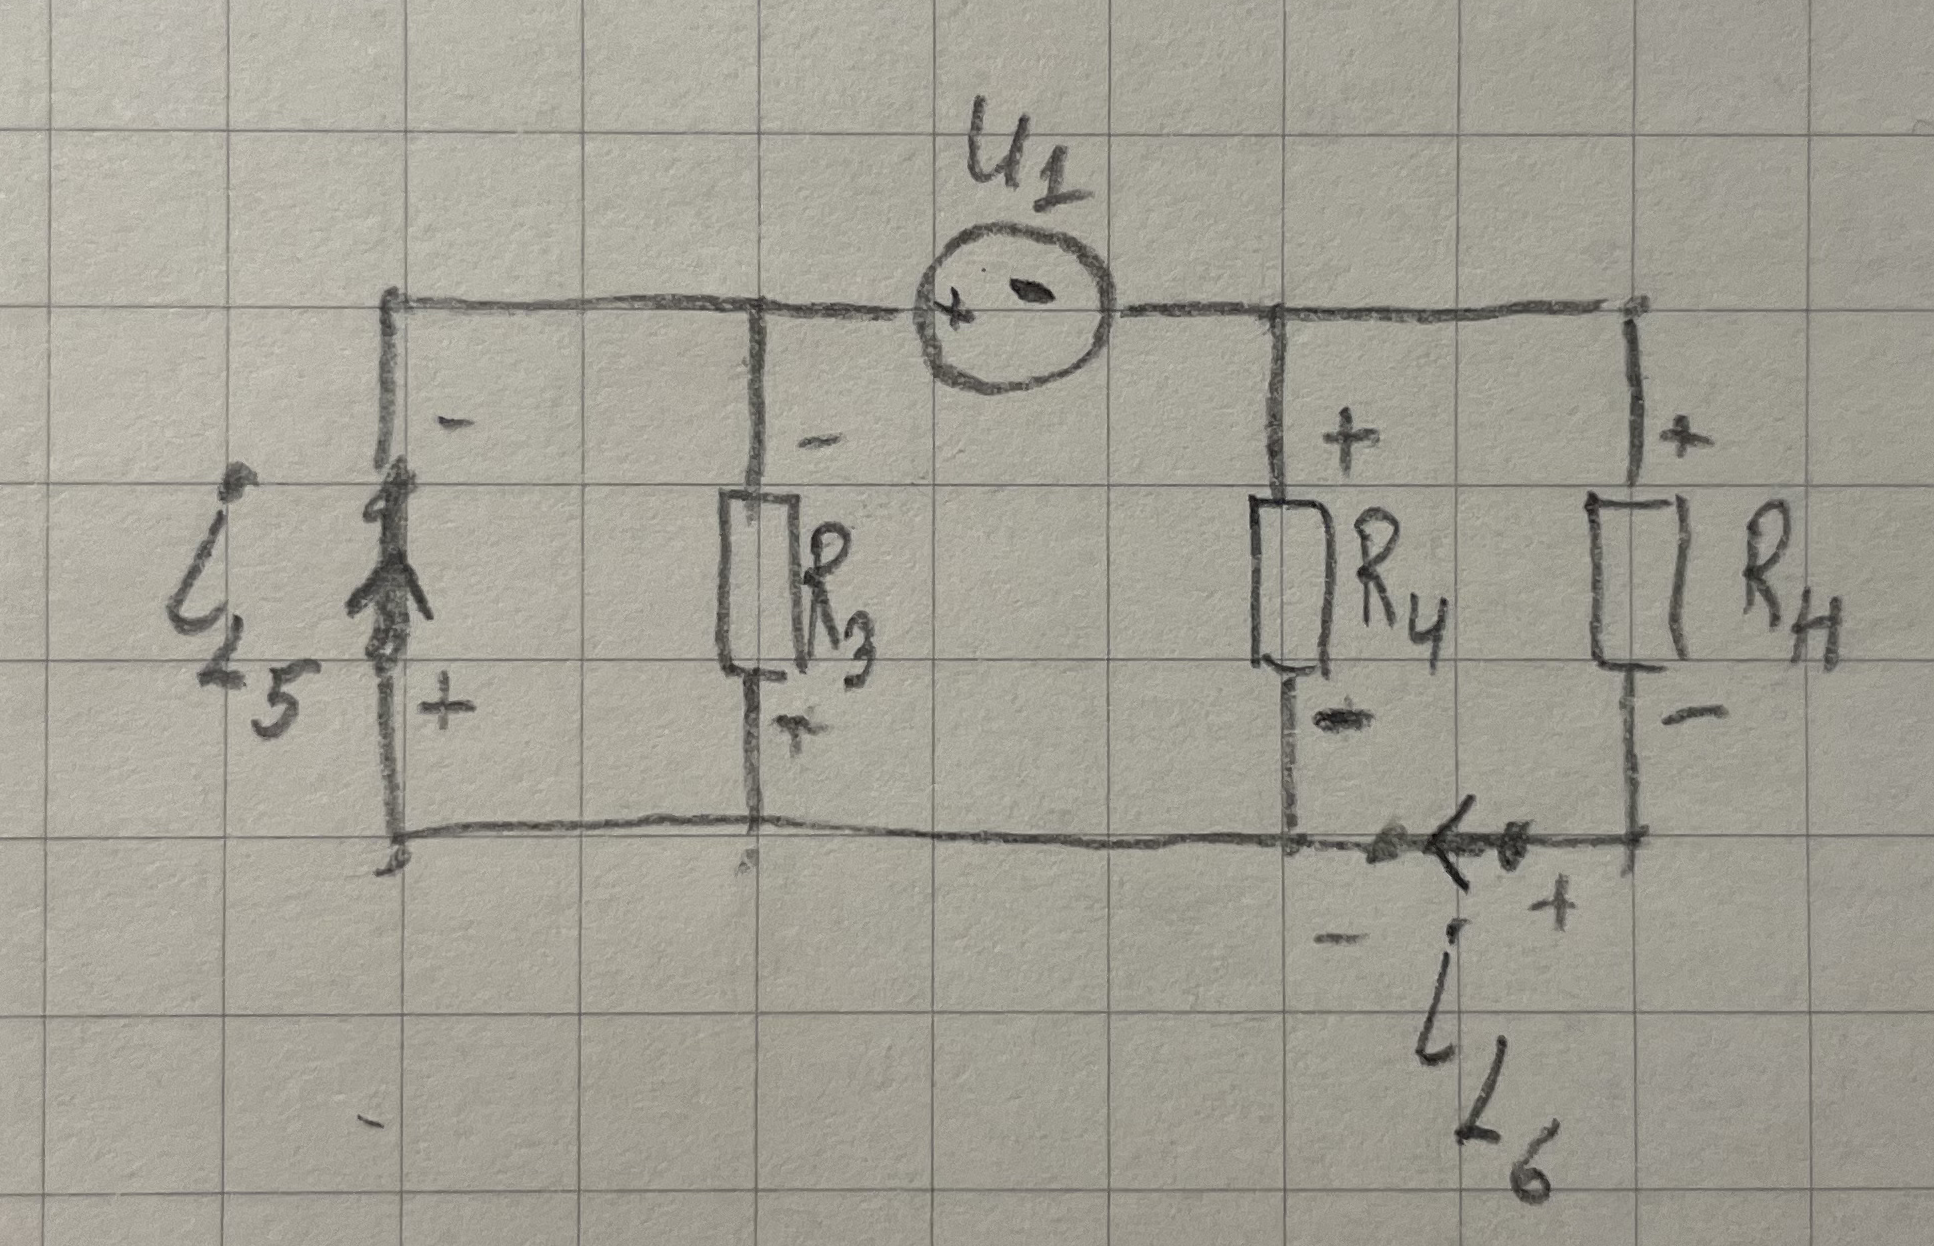
\includegraphics[width=0.7\linewidth]{photo/circ_replaced_2}
    \caption{Схема замещения. $ t \rightarrow \infty $}
    \label{fig:circ_replaced_2}
\end{figure}

$ i_{L_5 уст.} = 
i_{R_4} + i_{R_н} = 
\dfrac{u_{R_4}}{R_4} + \dfrac{u_{R_н}}{R_н} = 
\dfrac{u_1}{R_4} + \dfrac{u_1}{R_н} = 
\dfrac{1}{2} + \dfrac{1}{1} = 1.5
$

\begin{equation}\label{eq:i_L_6_}
i_{L_6 уст.} = i_{R_н} = 1
\end{equation}\\

Таким образом:

$ i_{L_5}(t) = 
A_1 e^{2t} \cos(t\sqrt{2}) + 
A_2 e^{2t} \sin(t\sqrt{2}) +
1.5
$

$ i_{L_6}(t) = 
B_1 e^{2t} \cos(t\sqrt{2}) + 
B_2 e^{2t} \sin(t\sqrt{2}) + 
1
$\\

По условию ННУ нулевые, поэтому:

$ i_{L_5}(0^-) = i_{L_5}(0^+) = 0 $

$ i_{L_6}(0^-) = i_{L_6}(0^+) = 0 $\\

Найдём постоянные интегрирования $ A_1, A_2 $:\\

$ \begin{cases}
    i_{L_5}(0^+) = 
    A_1 e^{2 \cdot 0^+} \cos(0^+ \cdot \sqrt{2}) + 
    A_2 e^{2 \cdot 0^+} \sin(0^+ \cdot \sqrt{2}) + 
    1.5\\
    i'_{L_5}(0^-) = 
    (2 A_2 - A_1 \sqrt{2}) e^{2 \cdot 0^-} \sin(0^- \cdot \sqrt{2}) +
    (A_2 \sqrt{2} + 2 A_1) e^{2 \cdot 0^-} \cos(0^- \cdot \sqrt{2})
\end{cases} $\\\\

$ \begin{cases}
    0 = A_1 \cdot 1 \cdot 1 + A_2 \cdot 1 \cdot 0 + 1.5\\
    0 = (2 A_2 - A_1 \sqrt{2}) \cdot 1 \cdot 0 + (A_2 \sqrt{2} + 2 A_1) \cdot 1 \cdot 1
\end{cases} $\\\\

$ \begin{cases}
    0 = A_1 + 1.5\\
    0 = A_2 \sqrt{2} + 2 A_1
\end{cases} $\\\\

$ \begin{cases}
    A_1 = - 1.5\\
    A_2 = \dfrac{3\sqrt{2}}{2}
\end{cases} $\\\\

Найдём постоянные интегрирования $ B_1, B_2 $:\\


$ \begin{cases}
    i_{L_6}(0^+) = 
    B_1 e^{2 \cdot 0^+} \cos(0^+ \cdot \sqrt{2}) + 
    B_2 e^{2 \cdot 0^+} \sin(0^+ \cdot \sqrt{2}) + 
    1\\
    i'_{L_6}(0^-) = 
    (2 B_2 - B_1 \sqrt{2}) e^{2 \cdot 0^-} \sin(0^- \cdot \sqrt{2}) +
    (B_2 \sqrt{2} + 2 B_1) e^{2 \cdot 0^-} \cos(0^- \cdot \sqrt{2})
\end{cases} $\\\\

$ \begin{cases}
    0 = B_1 \cdot 1 \cdot 1 + B_2 \cdot 1 \cdot 0 + 1\\
    0 = (2 B_2 - B_1 \sqrt{2}) \cdot 1 \cdot 0 + (B_2 \sqrt{2} + 2 B_1) \cdot 1 \cdot 1
\end{cases} $\\\\

$ \begin{cases}
    0 = B_1 + 1\\
    0 = B_2 \sqrt{2} + 2 B_1
\end{cases} $\\\\

$ \begin{cases}
    B_1 = -1\\
    B_2 = \sqrt{2}
\end{cases} $\\\\

Таким образом:

\begin{equation}\label{eq:i_L_5}
i_{L_5}(t) = 
- 1.5                e^{2t} \cos(t\sqrt{2}) + 
\dfrac{3\sqrt{2}}{2} e^{2t} \sin(t\sqrt{2}) +
1.5
\end{equation}

\begin{equation}\label{eq:i_L_6}
i_{L_6}(t) = 
-        e^{2t} \cos(t\sqrt{2}) + 
\sqrt{2} e^{2t} \sin(t\sqrt{2}) + 
1
\end{equation}

Из схемы на рис.\ref{fig:circ_source} следует, 
что реакция цепи $ i_н = i_{L_6} $,
тогда выражение переходной характеристики $ h_1(t) $
выходной реакции:

\begin{equation}\label{eq:h_1_t_1}
    h_1(t) = 
    (- e^{2t} \cos(t\sqrt{2}) + 
    \sqrt{2} e^{2t} \sin(t\sqrt{2}) + 1)\delta_1(t)
\end{equation}

На рис. \ref{fig:h_1_t} приведен график $ h_1(t) $.

\begin{figure}[H]
    \centering
    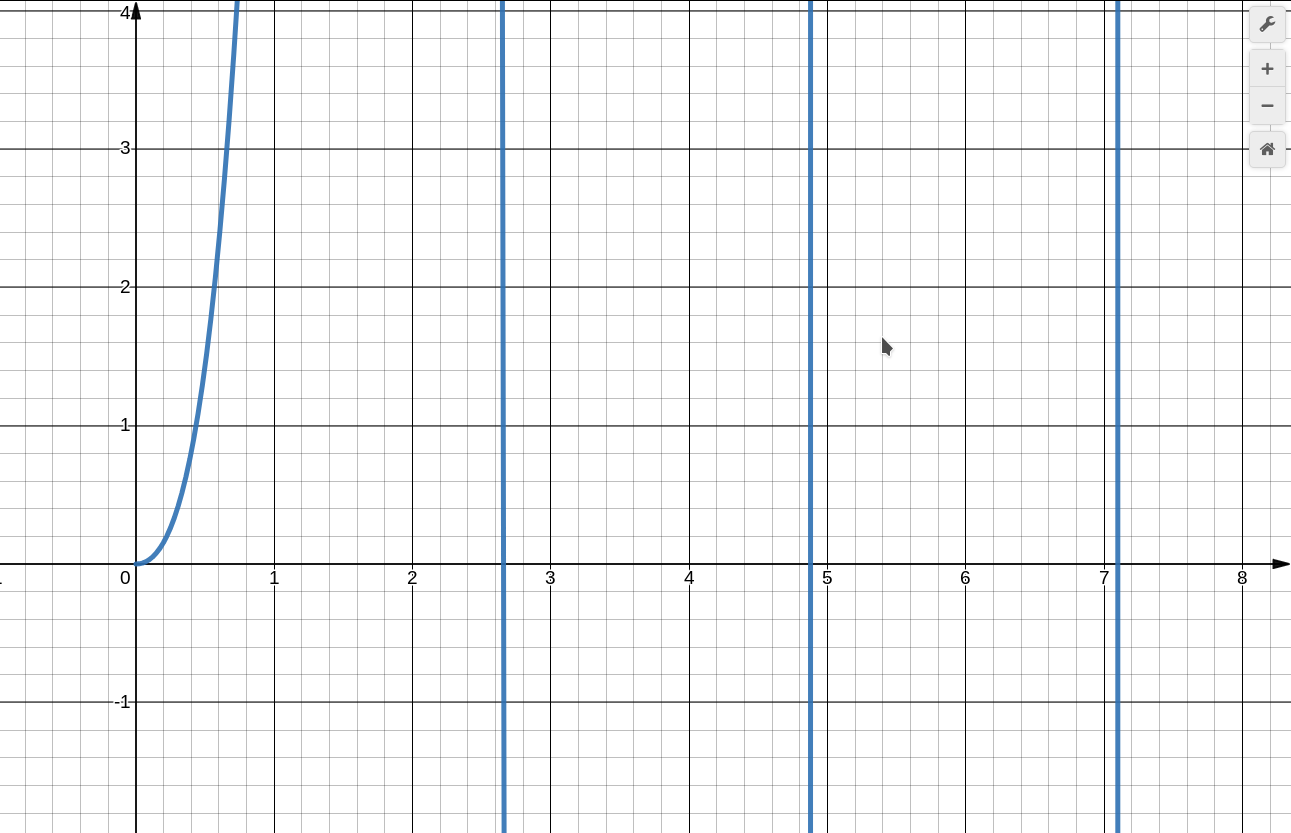
\includegraphics[width=0.7\linewidth]{photo/h_1_t}
    \caption{График $ h_1(t) $}
    \label{fig:h_1_t}
\end{figure}